	\subsection{Indstillinger}
	Dette afsnit vil indeholde en gennem gang af design, grafisk bruger interface og implentering af Indstilinger activityen til android applikationen
	
	\subsubsection{Design}
	
	\subsubsection{Grafisk Bruger Interface}	
	Visning af det graiske bruger interface når man vælger indstillinger
	\begin{figure} [!ht]
		\begin{center}
			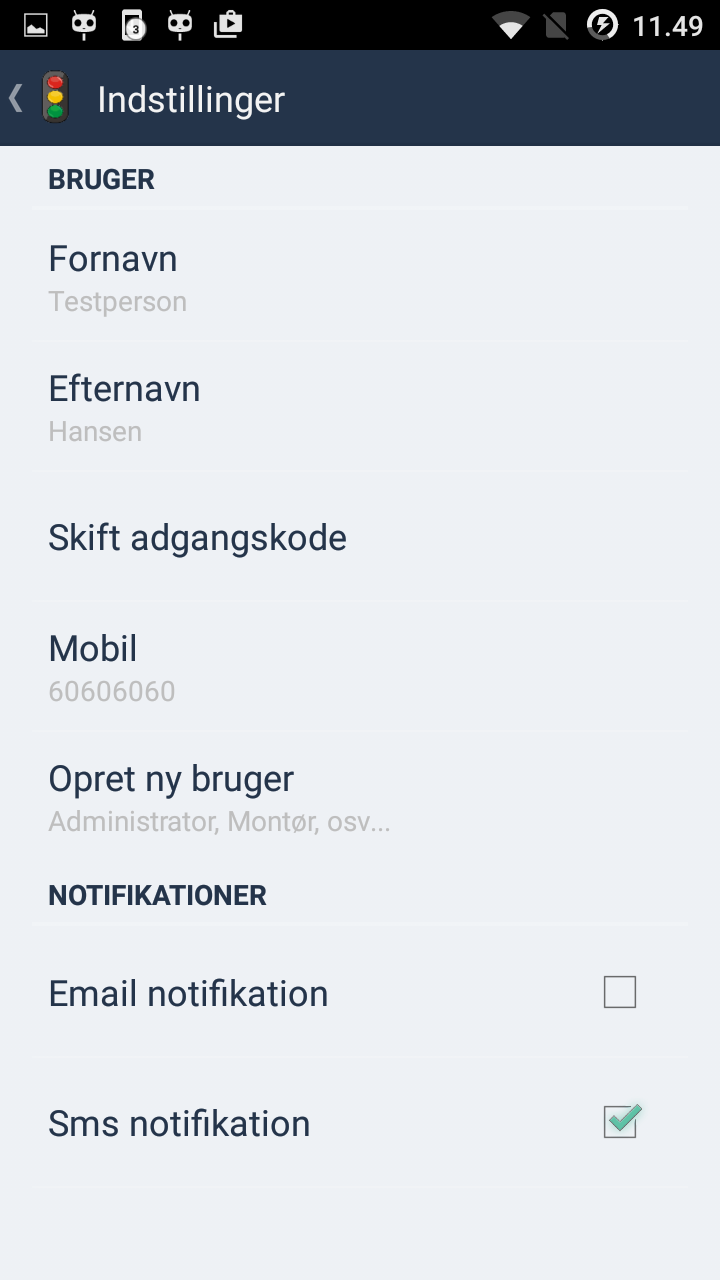
\includegraphics[height=10cm]{Android/Billeder/AndroidInstillinger}
		\end{center}
		\caption{Instillinger på android applikationen}
		\label{fig:Instillinger på android applikationen}
	\end{figure} \\
	Vælges der indstillinger kommer man ind på ovenstående skærm. Her har man mulighed for at ændre oplysninger for sin egen bruger, i form af navn, mobilnummer og adgangskode. Man har også mulighed for at vælge om man ønsker notifikationer og hvordan man ønsker disse notifikationer.
	
	\subsubsection{Implementering}
	
	\pagebreak